This component is responsible for maintaining a list of pending OutComponents and for repeatedly executing them until they are serialized and sent to their destination.
The list of pending commands is called the \textit{Pending OutComponent List} or POCL. The POCL has a fixed size which is defined when the OutManager is initialized. 

The OutManager component offers a \texttt{Load} operation through which an OutComponent can be added to the POCL (see activity diagram in figure \ref{fig:OutManagerLoad}). This operation is called by the OutLoader of the previous section. The \texttt{Load} operation may fail if the list is full. In this case, the OutComponent is released. This protects the application against resource leaks in case of repeated \texttt{Load} failures.

The \texttt{Load} operation registers the newly loaded OutComponent with the OutRegistry using its StartTracking operation (see figure \ref{fig:RegistryStartTracking}). Henceforth, and as long as the OutComponent remains loaded in the OutManager, its state is tracked by the OutRegistry. 

\begin{figure}[h]
 \centering
 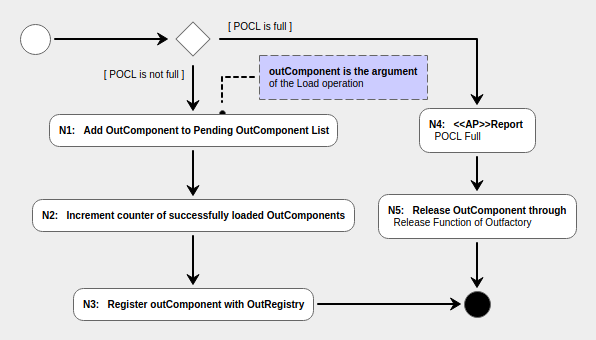
\includegraphics[scale=0.5,keepaspectratio=true]{OutManagerLoad.png}
 \caption{The OutManager Load Procedure}
 \label{fig:OutManagerLoad}
\end{figure}

The OutComponents loaded into the POCL must be fully configured (i.e. they must be in state CONFIGURED). It is the responsibility of the user of the OutManager to ensure that this constraint is complied with. Note that, since OutComponents are loaded into the OutManager by the OutLoader (see previous section), this constraint must be enforced by the host application when it loads an out-going command or report into the OutLoader. Violation of this constraint will result in an OutComponent permanently remaining in the POCL of the OutManager.

The OutManager maintains a counter of successfully loaded OutComponents. The counter is initialized to zero when the OutManager is reset.

The order in which the items in the POCL are processed by the OutManager is unspecified.

There is no mechanism to “unload” a pending OutComponent. The OutManager autonomously returns an OutComponent to the OutFactory when the OutComponent has been sent to its destination (i.e. when the OutComponent is in state TERMINATED) or when it has been aborted (i.e. when the OutComponent is in state ABORTED). 

\begin{figure}[h]
 \centering
 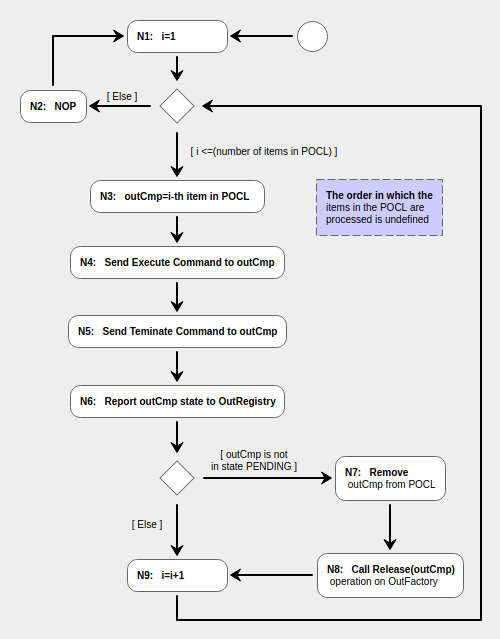
\includegraphics[scale=0.5,keepaspectratio=true]{OutManagerExecution.png}
 \caption{The OutManager Execution Procedure}
 \label{fig:OutManagerExecution}
\end{figure}

The OutManager component is defined as an extension of the Base Component of section \ref{sec:BaseCmp}. It uses the \textit{Execution Procedure} of the Base Component to process the pending commands. The OutManager component processes the pending commands by sending them an \texttt{Execute} command. After each \texttt{Execute} command, the state of the OutComponent is reported to the OutRegistry using the latter Update function (see figure \ref{fig:RegistryUpdate}). Commands which have been aborted or have been sent to their destination are removed from the POCL and are returned to the OutFactory. The \textit{Execution Procedure} of the OutManager is shown in figure \ref{fig:OutManagerExecution}.

Normally, the OutManager is embedded within a Real Time Container (see reference [FW-SP]) which is responsible for executing it. Thus, an application that is required to process out-going commands or reports at different levels of priority should use several OutManagers (one for each level of priority) and should allocate them to Real Time Containers with a matching priority.

